\section{Machine learning pipeline experiment}\label{appendix:ml-pipeline-experiment}
Het experiment is uitgevoerd om te valideren of de stappen van de ML pipeline valide zijn en om de stappen beter te begrijpen. Het machine learning probleem dat wordt gebruikt om de ML pipeline te testen is het iris probleem. Bij dit probleem hoort een dataset dat bestaat uit 150 samples van drie iris soorten: Setosa, Virginica en Versicolor. Elk voorbeeld heeft de lengte en breedte van de kelk- en bloemblad met de bijbehorende soort iris. In \autoref{table:example-iris-dataset} is een voorbeeld van de dataset te zien. Het model zal een van de drie soorten kunnen herkennen op basis van de lengte en breedte van een gegeven kelk- en bloemblad. 

\begin{table}[hbt!]
  \footnotesize
  \centering
  \begin{tabular}{|l|l|l|l|l|}
  \hline
  \textbf{Kelkblad - lengte} & \textbf{Kelkblad - breedte} & \textbf{Bloemblad - lengte} & \textbf{Bloemblad - breedte} & \textbf{Soort} \\ \hline
  5.1 & 3.5 & 1.4 & 0.2 & Iris-setosa\\ \hline
  \end{tabular}
  \caption{Voorbeeld van de iris dataset}
  \label{table:example-iris-dataset}
\end{table}

\begin{figure}[hbt!]
  \centering
  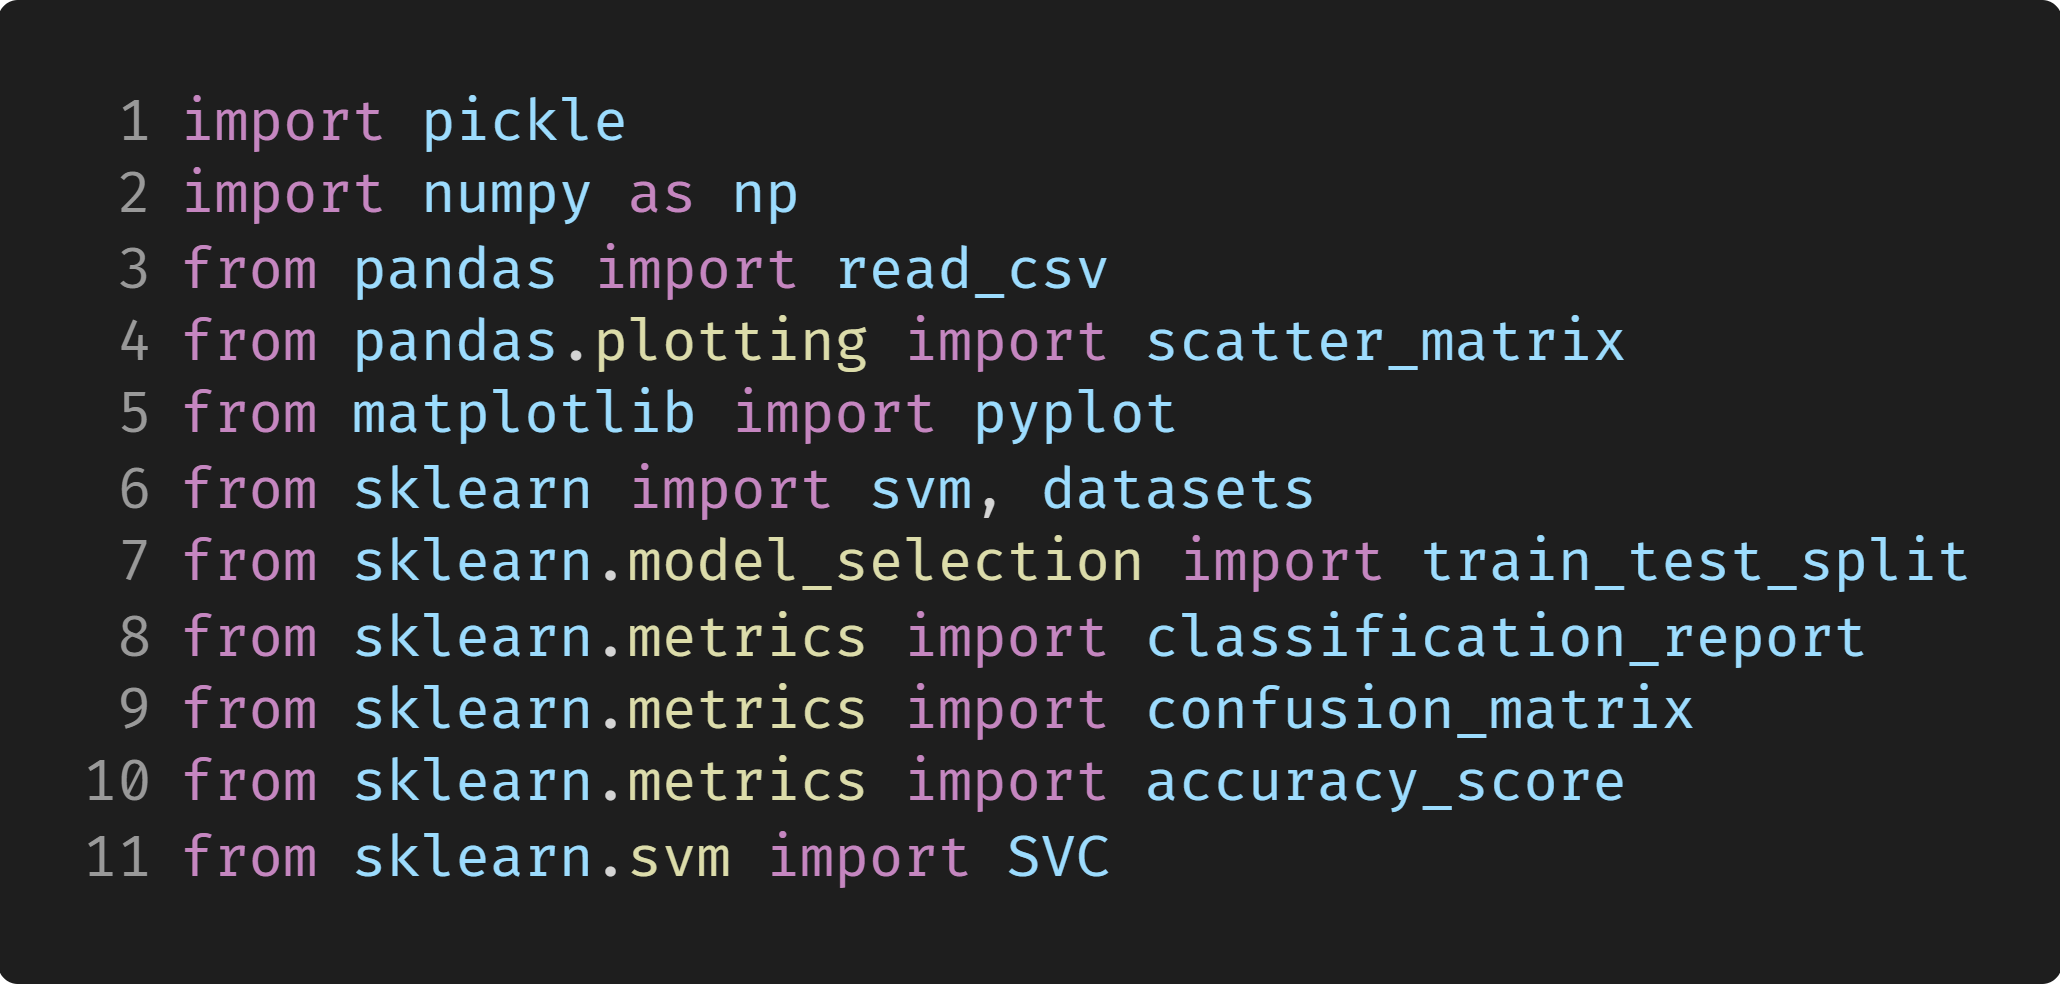
\includegraphics[width=0.6\textwidth]{ml-iris/ml-iris-imports.png}
  \caption{Importeren van modules}
  \label{fig:appendix:ml-iris-imports}
\end{figure}

\begin{figure}[hbt!]
  \centering
  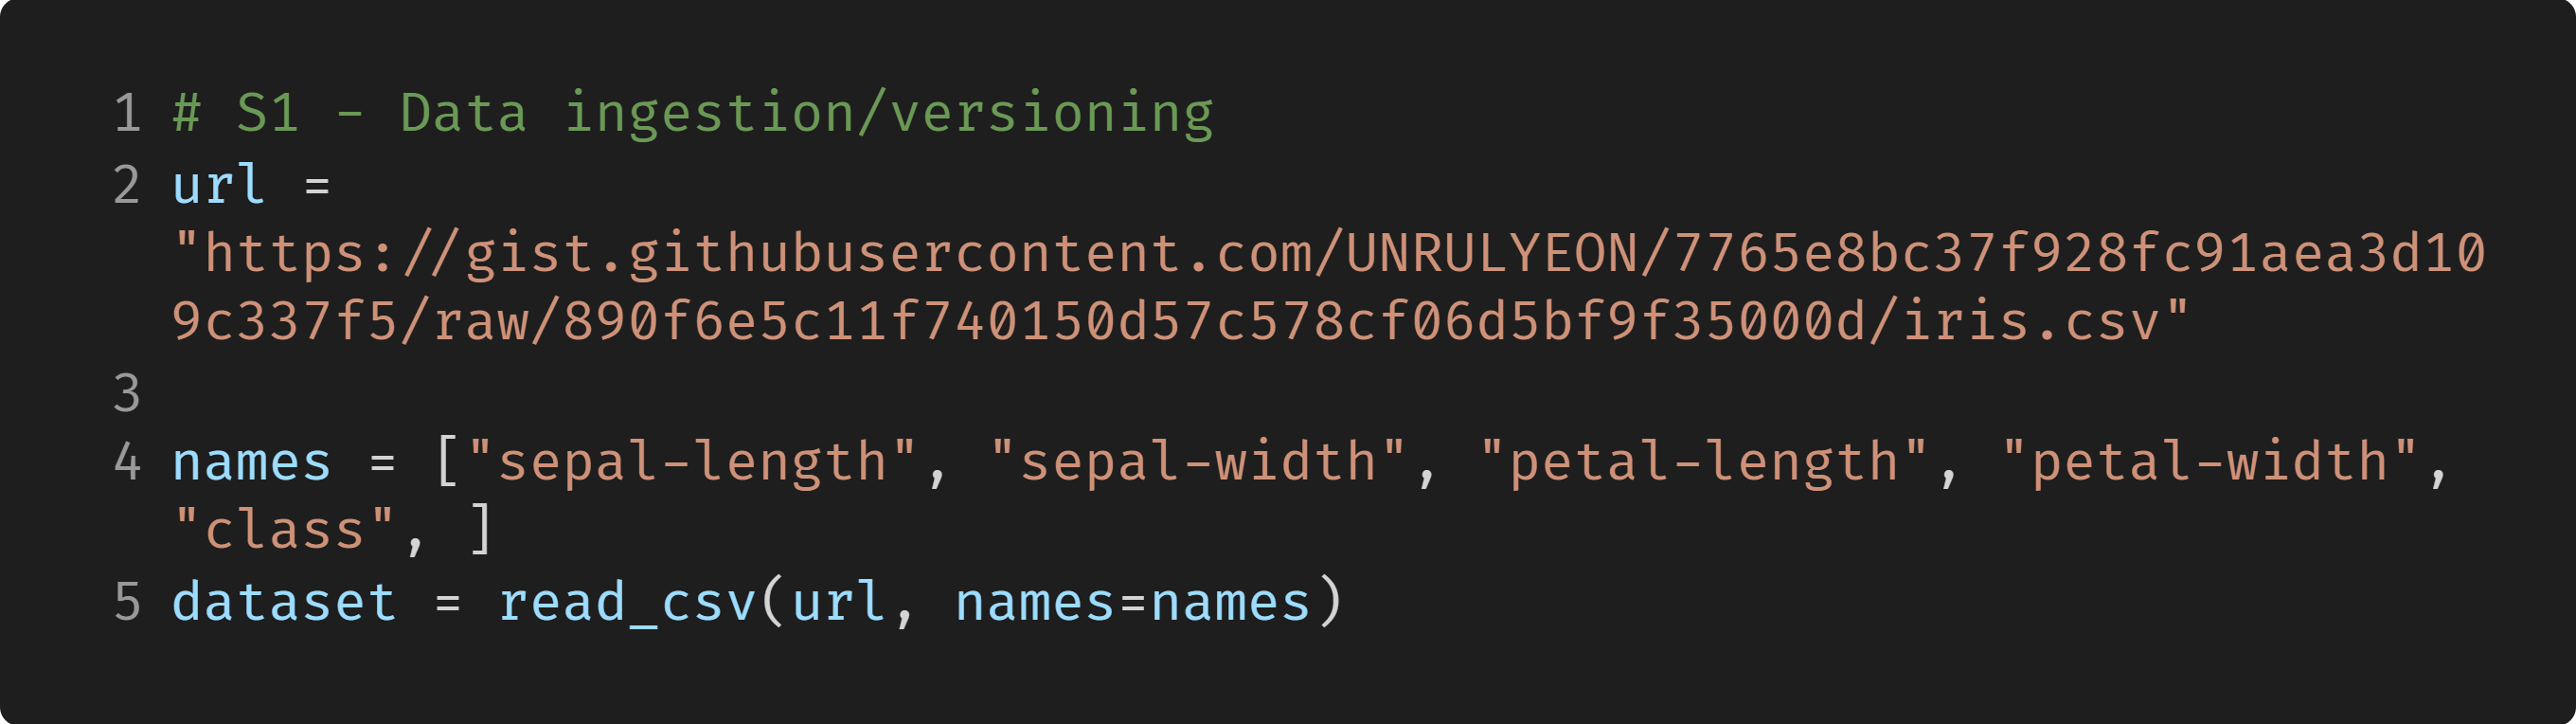
\includegraphics[width=0.8\textwidth]{ml-iris/ml-iris-1-import-dataset.png}
  \caption{Importeren van de dataset}
  \label{fig:appendix:ml-iris-1-import-dataset}
\end{figure}

\clearpage

\begin{figure}[hbt!]
  \centering
  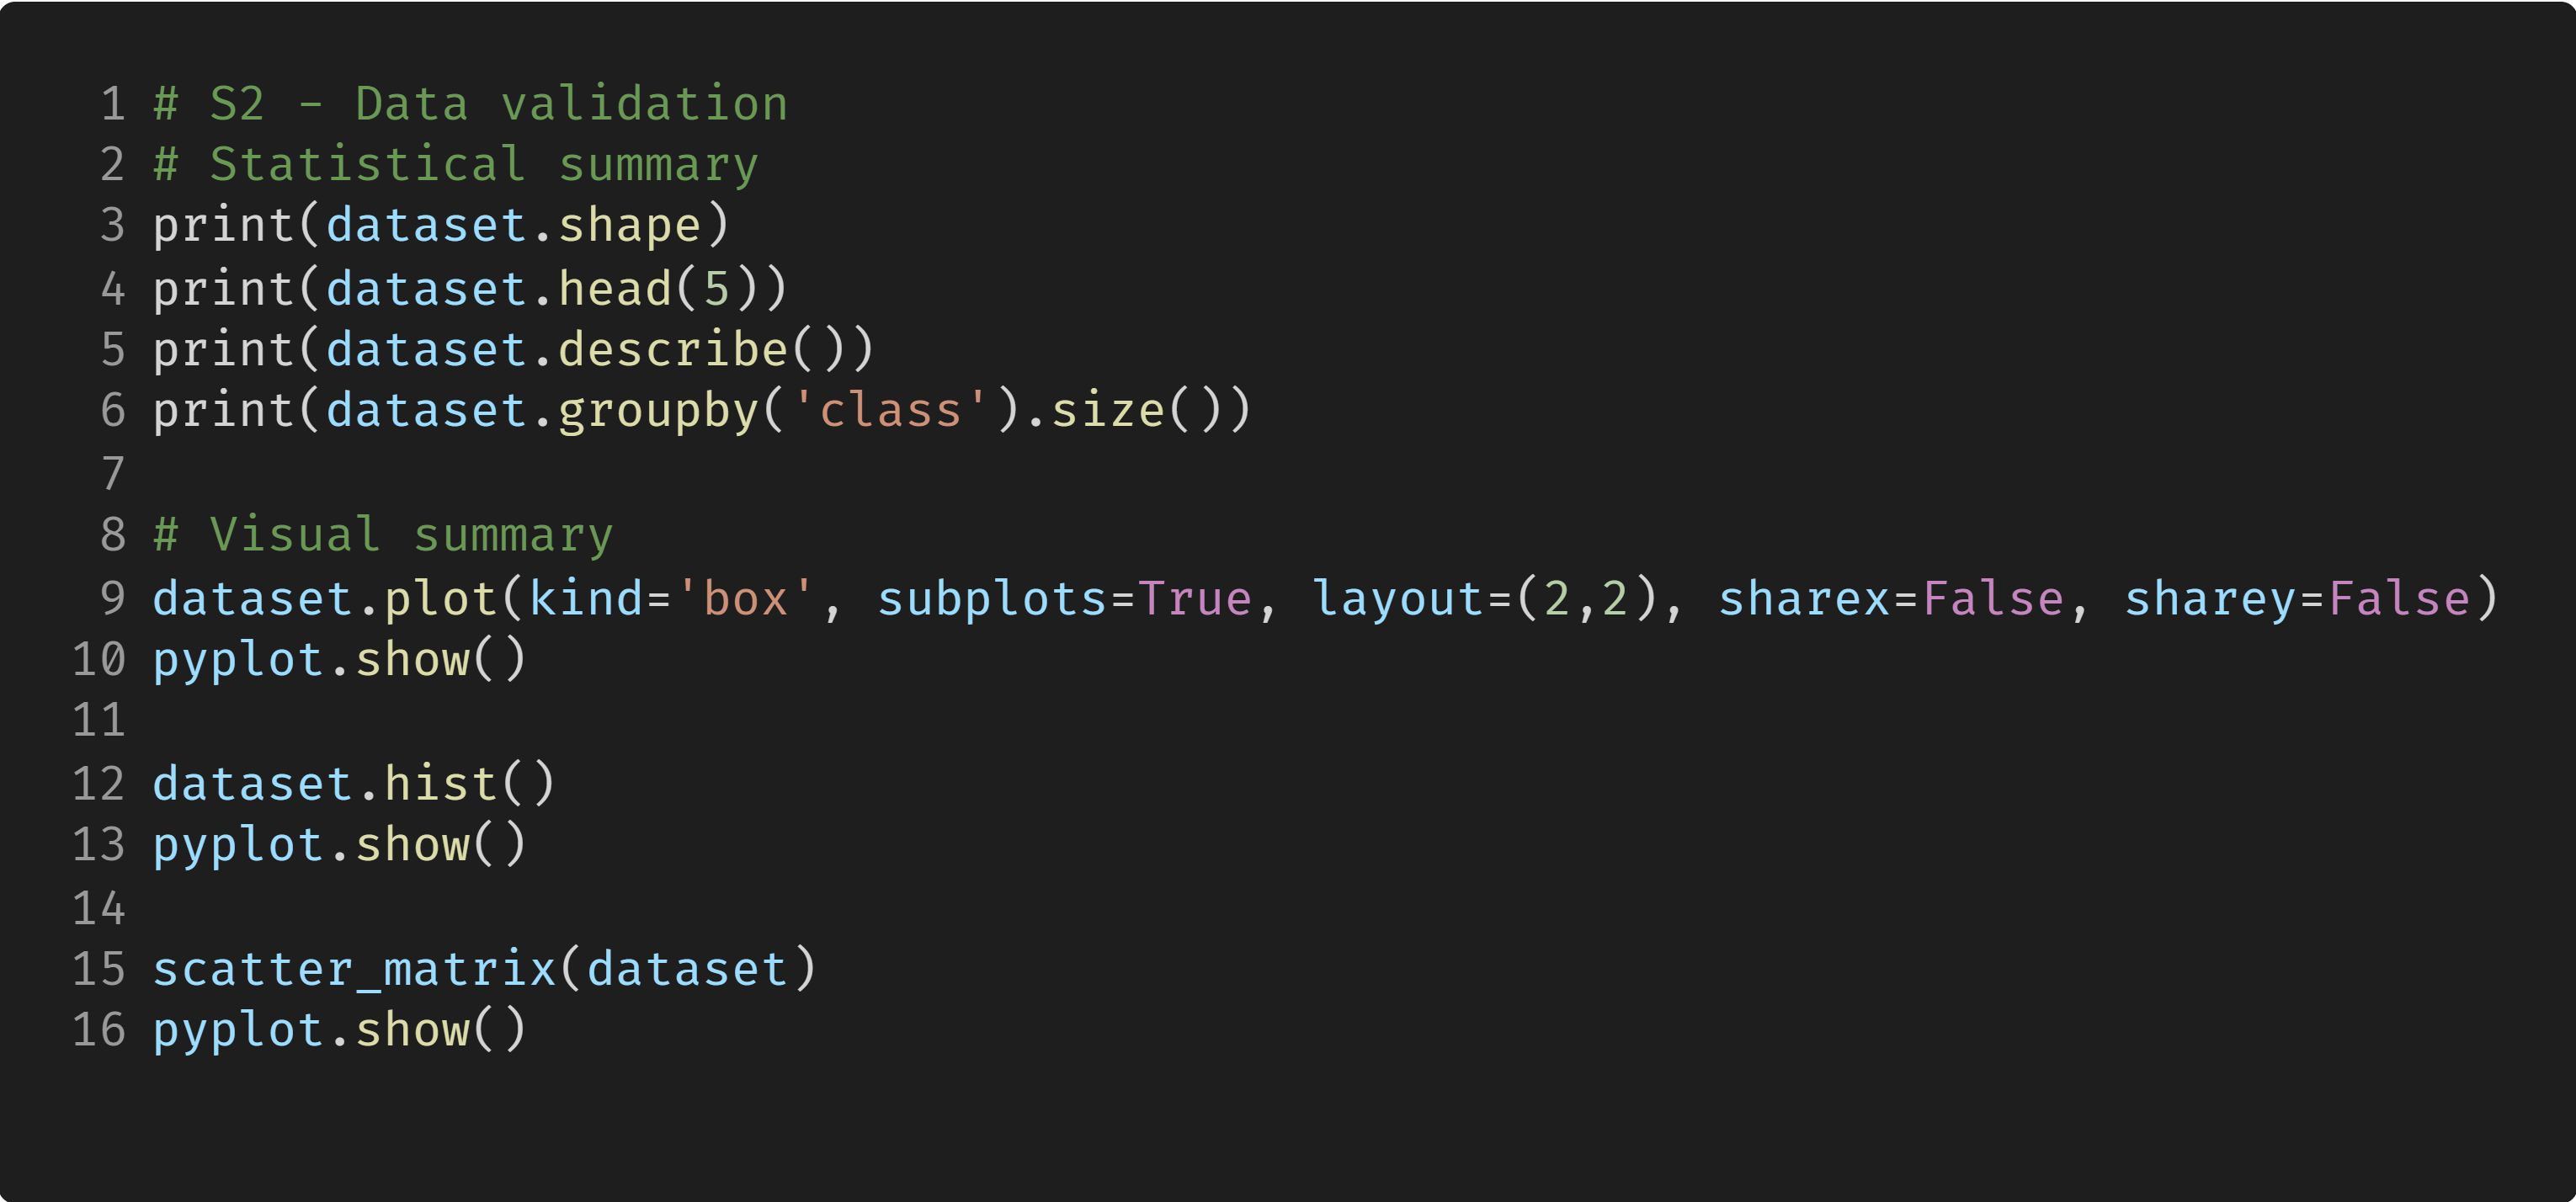
\includegraphics[width=0.8\textwidth]{ml-iris/ml-iris-2-data-validation.png}
  \caption{Validatie van de dataset}
  \label{fig:appendix:ml-iris-2-data-validation}
\end{figure}

\clearpage

\begin{figure}[hbt!]
  \centering
  \begin{minipage}{0.5\textwidth}
      \centering
      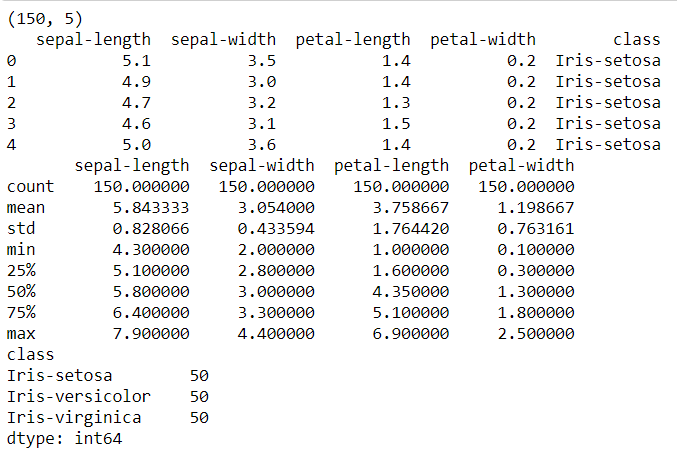
\includegraphics[width=0.9\textwidth]{ml-iris/ml-iris-2-data-validation-result-1.png}
      \caption{Validatie van de dataset - resultaat 1}
      \label{fig:appendix:ml-iris-2-data-validation-result-1}
  \end{minipage}\hfill
  \begin{minipage}{0.5\textwidth}
      \centering
      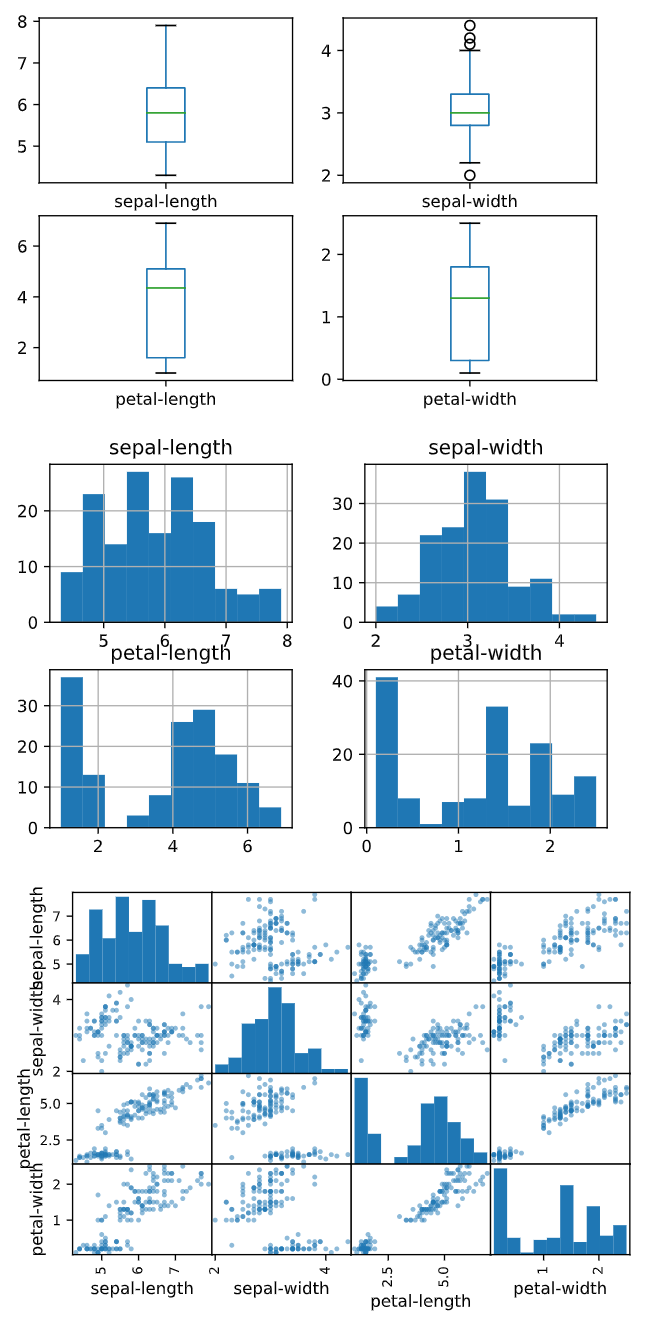
\includegraphics[width=0.9\textwidth]{ml-iris/ml-iris-2-data-validation-result-2.png}
      \caption{Validatie van de dataset - resultaat 2}
      \label{fig:appendix:ml-iris-2-data-validation-result-2}
  \end{minipage}
\end{figure}

\begin{figure}[hbt!]
  \centering
  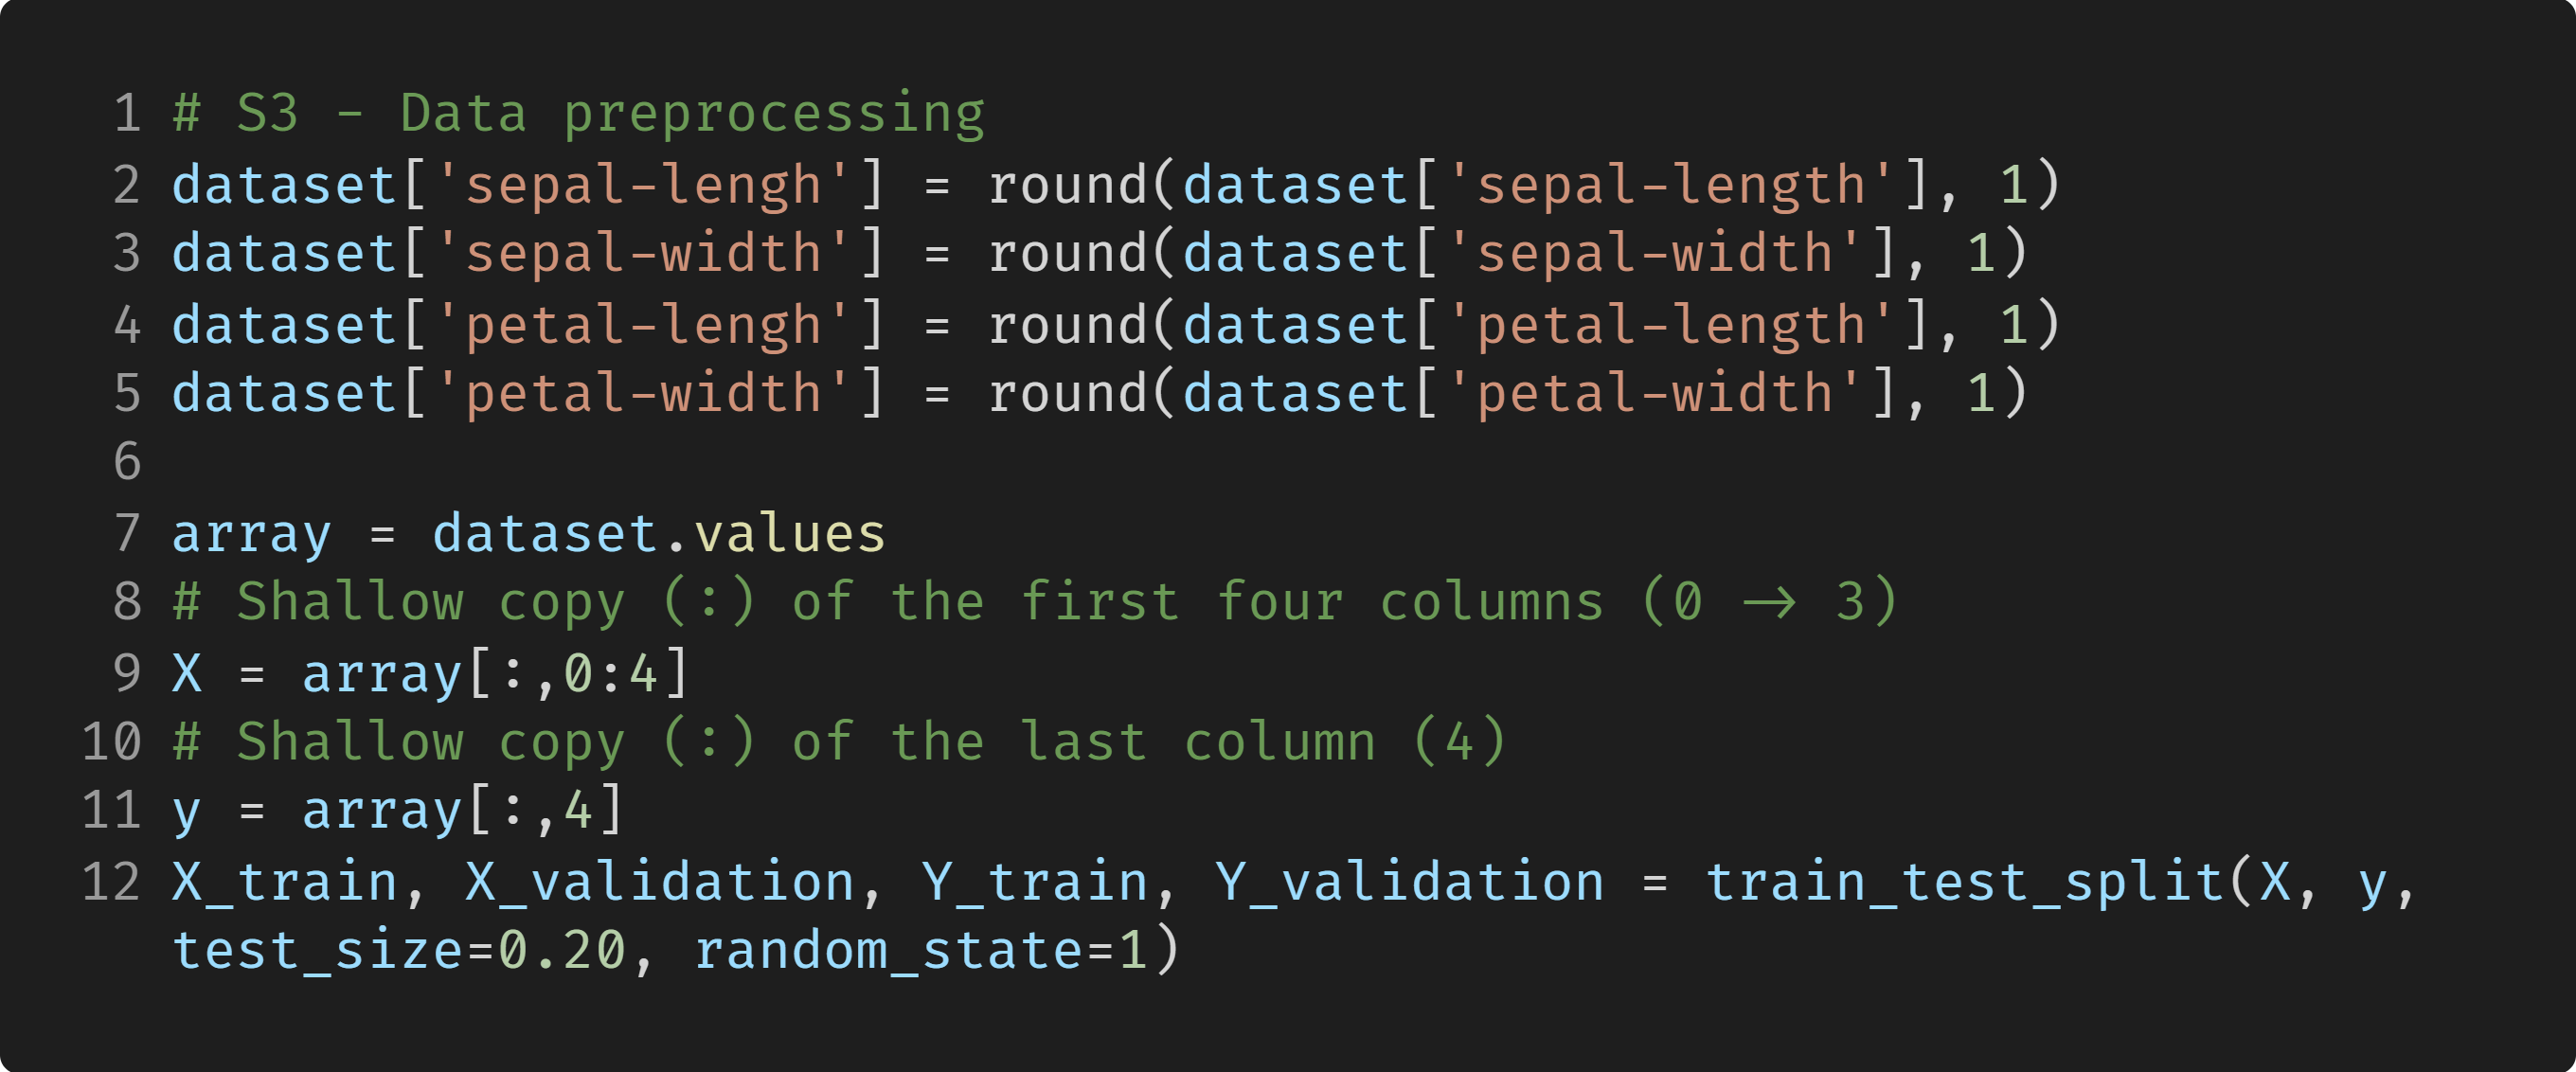
\includegraphics[width=0.71\textwidth]{ml-iris/ml-iris-3-data-preprocessing.png}
  \caption{Dataset voorbereiden}
  \label{fig:appendix:ml-iris-3-data-preprocessing}
\end{figure}

\begin{figure}[hbt!]
  \centering
  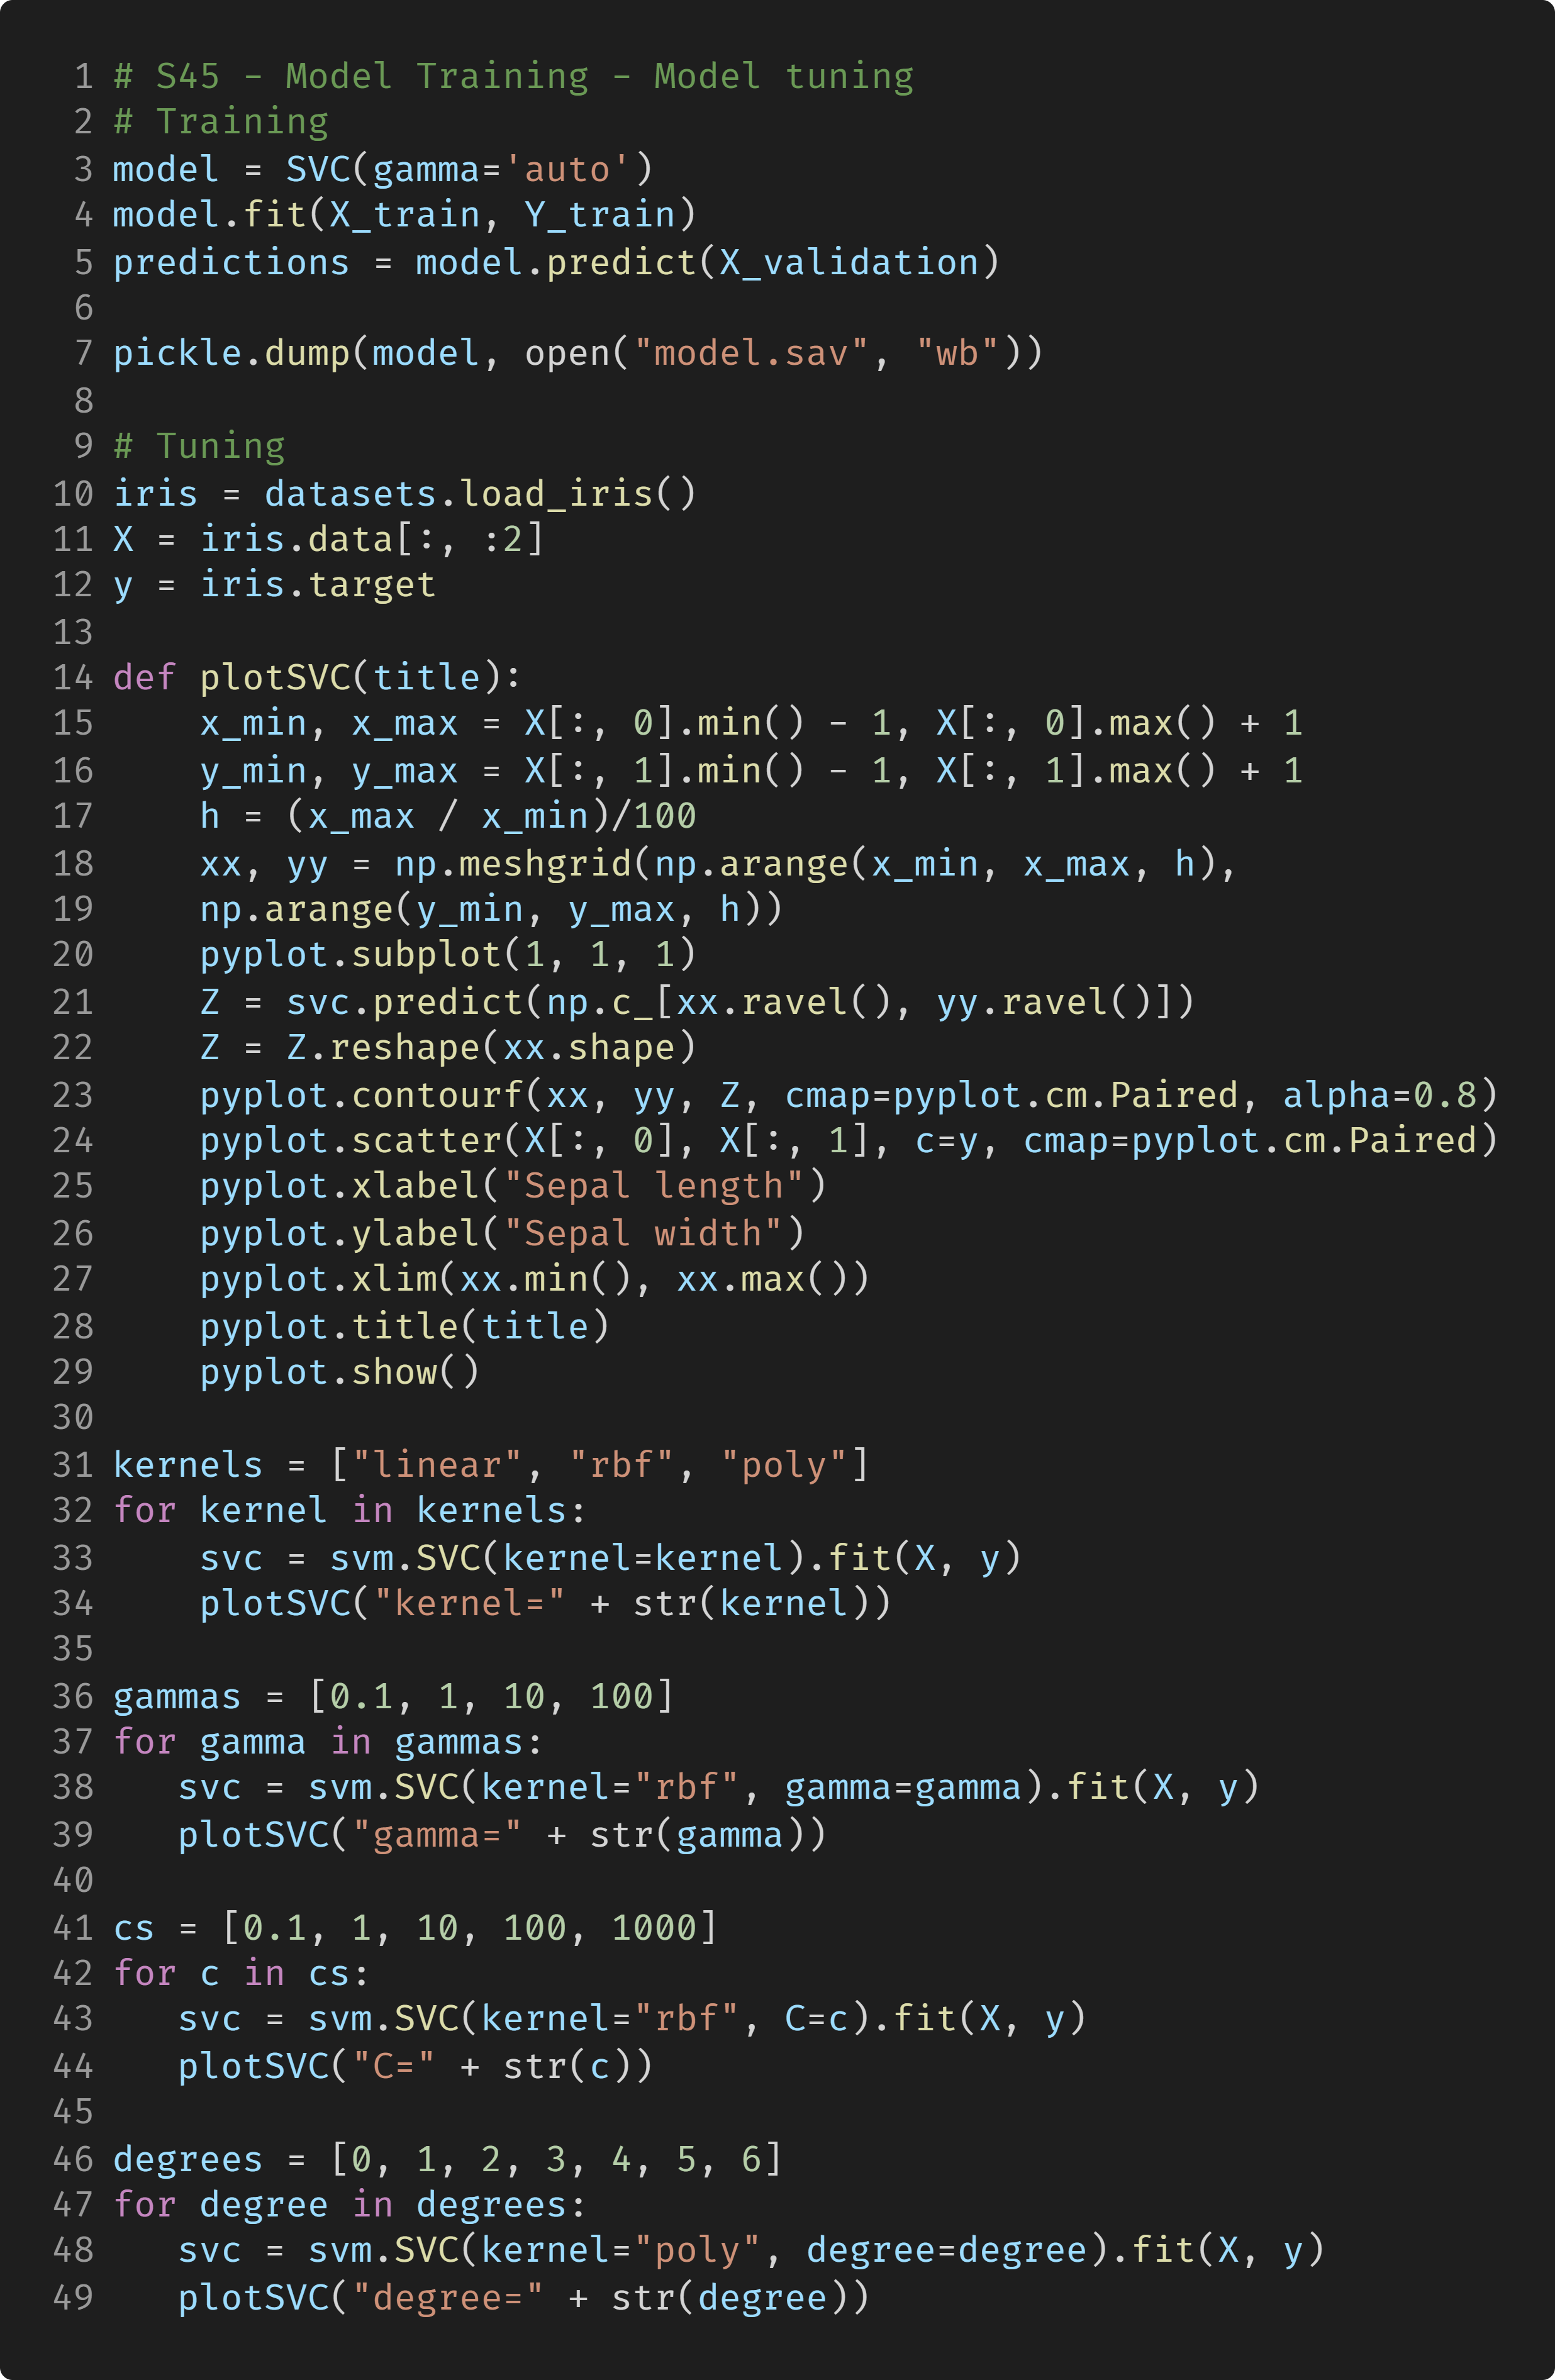
\includegraphics[width=0.8\textwidth]{ml-iris/ml-iris-45-model-training-model-tuning.png}
  \caption{Dataset voorbereiden}
  \label{fig:ml-iris-45-model-training-model-tuning}
\end{figure}

\clearpage

\begin{figure}[hbt!]
  \centering
  \begin{minipage}{0.45\textwidth}
      \centering
      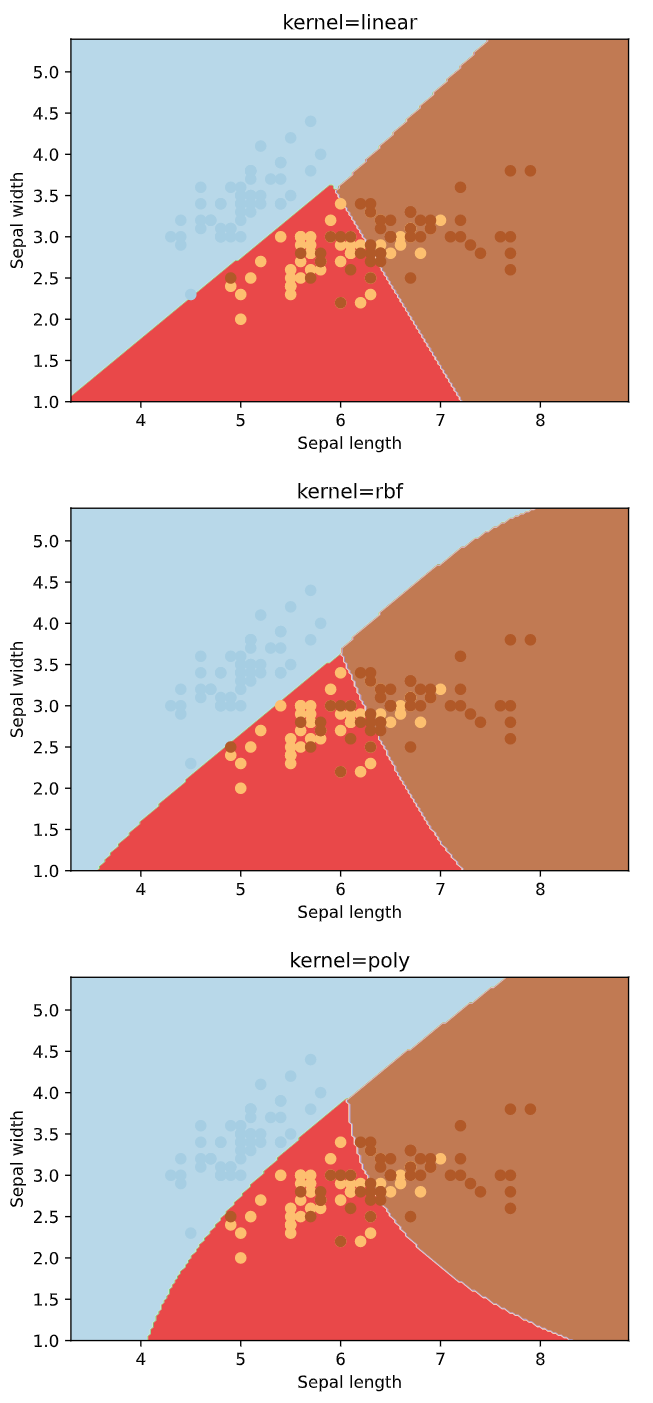
\includegraphics[width=1\textwidth]{ml-iris/ml-iris-45-model-training-model-tuning-kernel.png}
      \caption{Verschil van de kernel hyperparameter}
      \label{fig:appendix:ml-iris-45-model-training-model-tuning-kernel}
  \end{minipage}\hfill
  \begin{minipage}{0.45\textwidth}
      \centering
      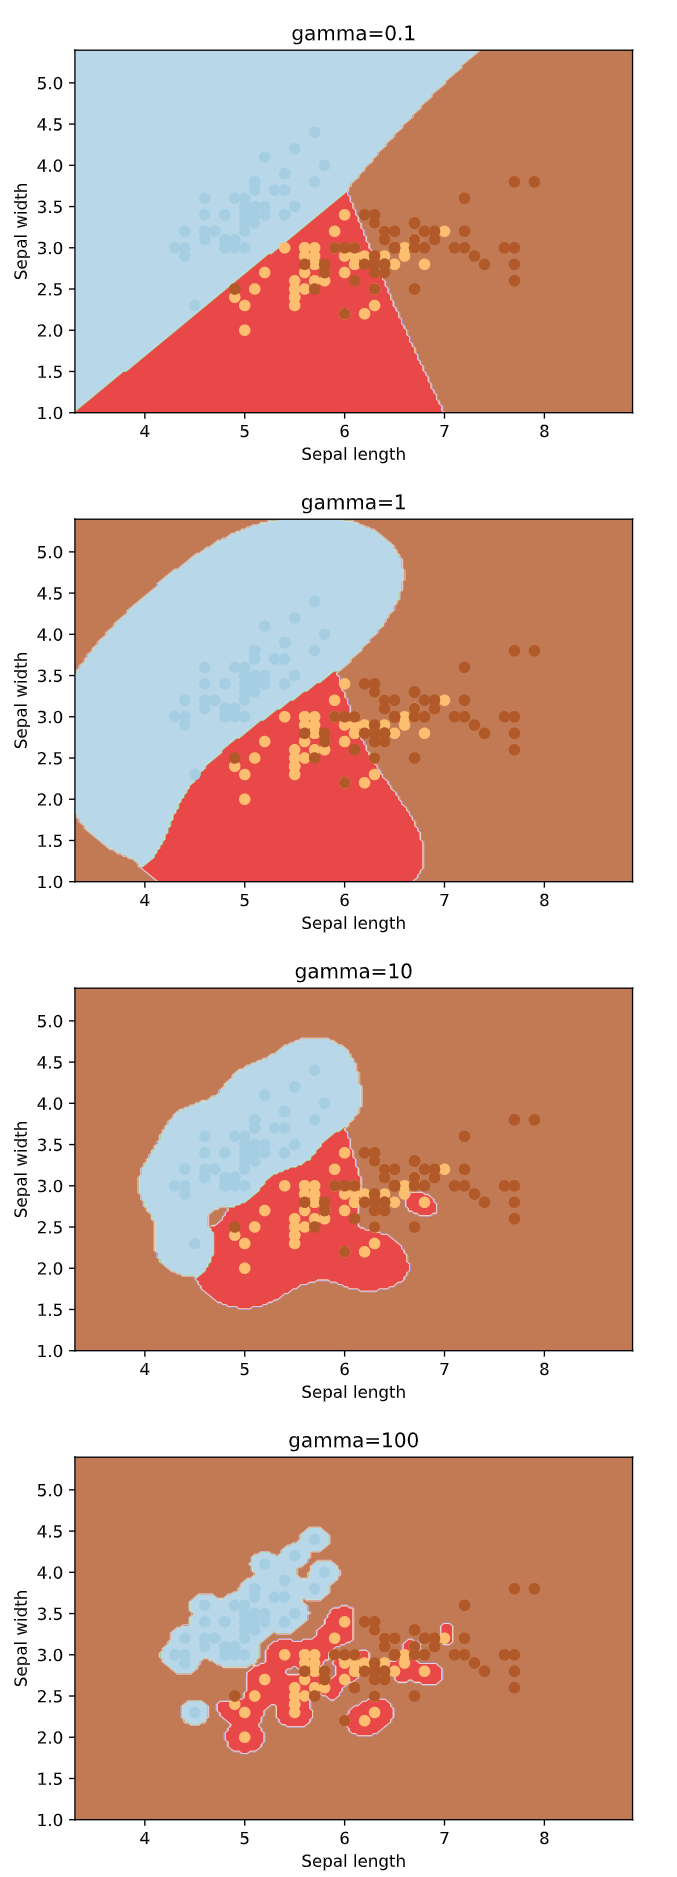
\includegraphics[width=1\textwidth]{ml-iris/ml-iris-45-model-training-model-tuning-gamma.png}
      \caption{Verschil van de gamma hyperparameter}
      \label{fig:appendix:ml-iris-45-model-training-model-tuning-gamma}
  \end{minipage}
\end{figure}

\clearpage

\begin{figure}[hbt!]
  \centering
  \begin{minipage}{.5\textwidth}
      \centering
      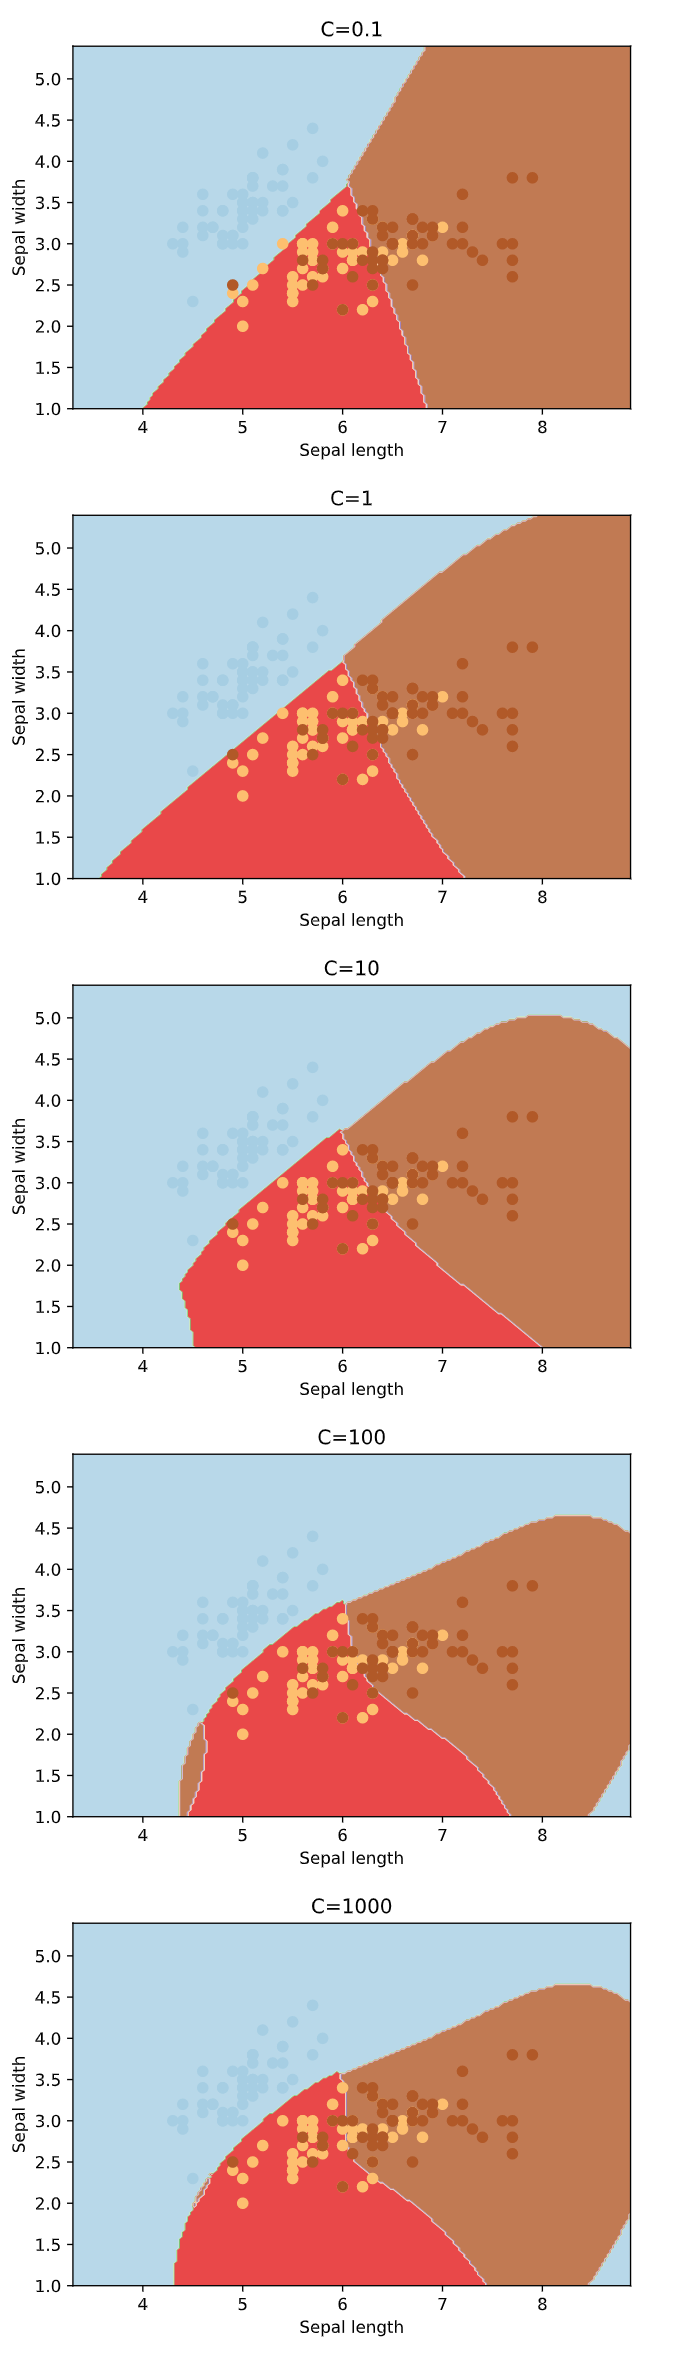
\includegraphics[width=.775\textwidth]{ml-iris/ml-iris-45-model-training-model-tuning-c.png}
      \caption{Verschil van de c hyperparameter}
      \label{fig:appendix:ml-iris-45-model-training-model-tuning-c}
  \end{minipage}\hfill
  \begin{minipage}{.5\textwidth}
      \centering
      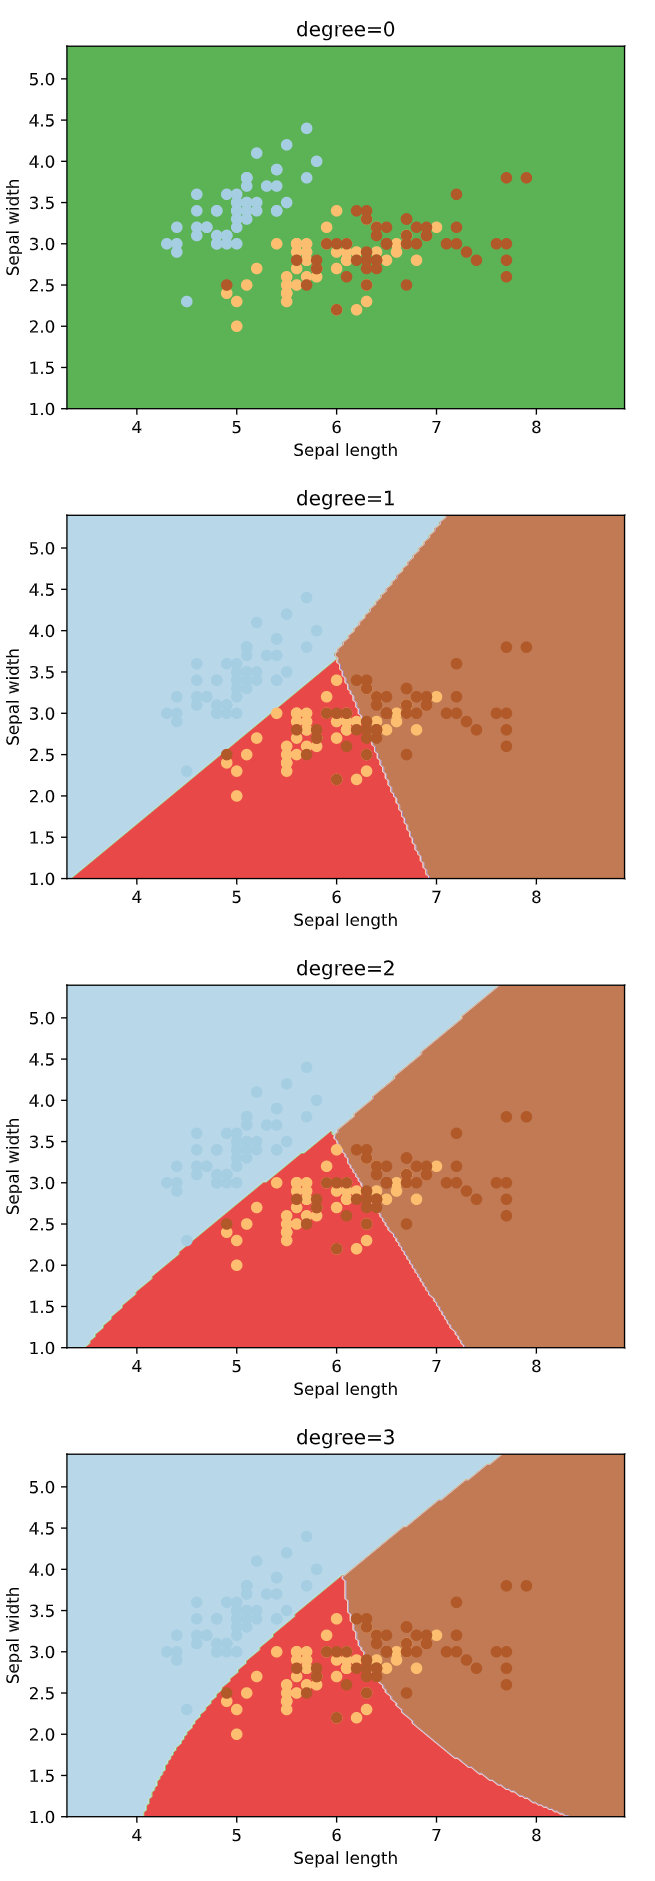
\includegraphics[width=.85\textwidth]{ml-iris/ml-iris-45-model-training-model-tuning-degree.png}
      \caption{Verschil van de degree hyperparameter}
      \label{fig:appendix:ml-iris-45-model-training-model-tuning-degree}
  \end{minipage}
\end{figure}

\clearpage

\begin{figure}[hbt!]
  \centering
  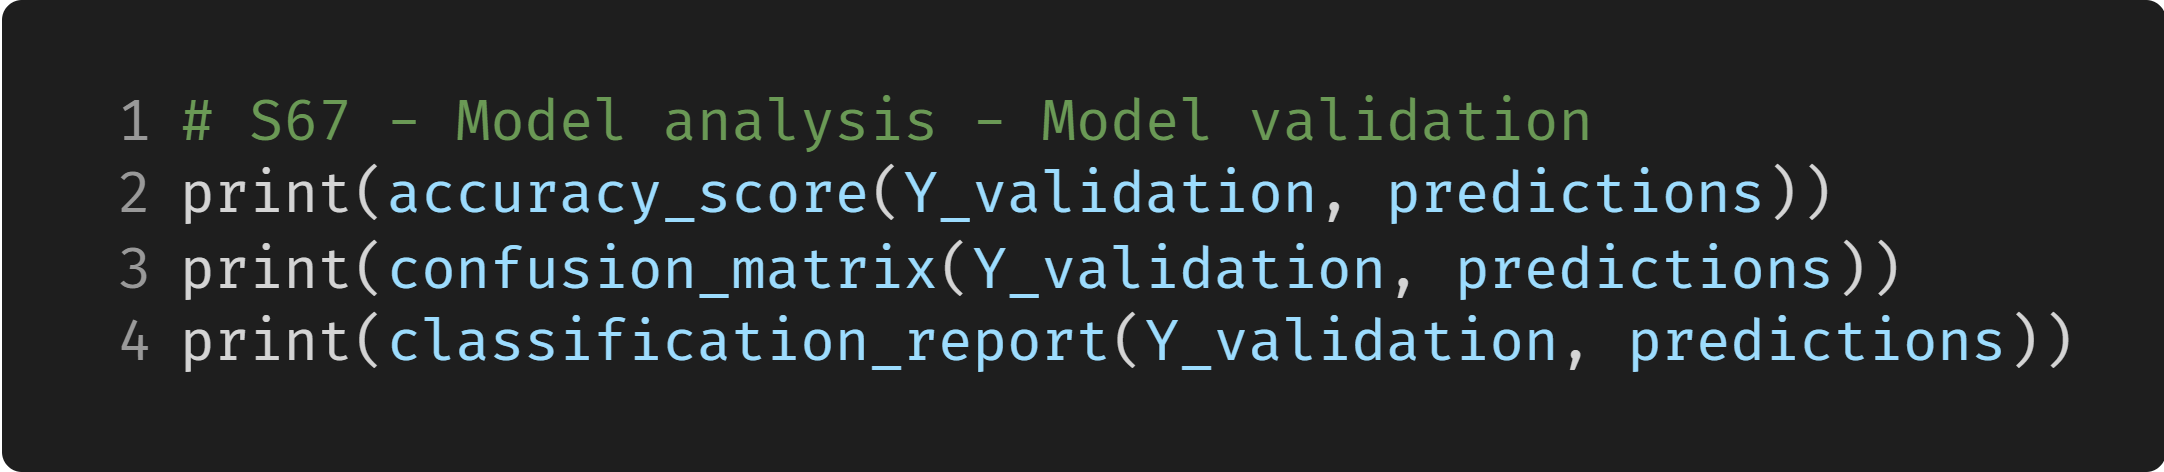
\includegraphics[width=0.8\textwidth]{ml-iris/ml-iris-67-model-analysis-model-validation.png}
  \caption{Dataset voorbereiden}
  \label{fig:appendix:ml-iris-67-model-analysis-model-validation}
\end{figure}

\begin{figure}[hbt!]
  \centering
  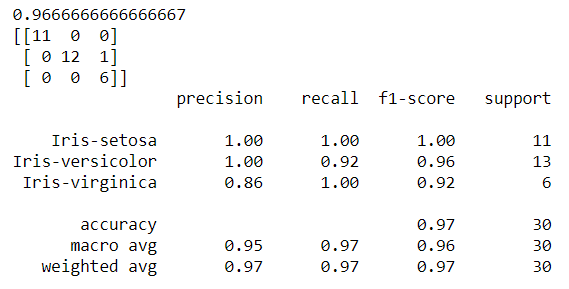
\includegraphics[width=0.8\textwidth]{ml-iris/ml-iris-67-model-analysis-model-validation-result.png}
  \caption{Dataset voorbereiden}
  \label{fig:appendix:ml-iris-67-model-analysis-model-validation-result}
\end{figure}

\newpage